\section{Motivation}
\label{motivation}


\begin{figure}[t]
	\centering
	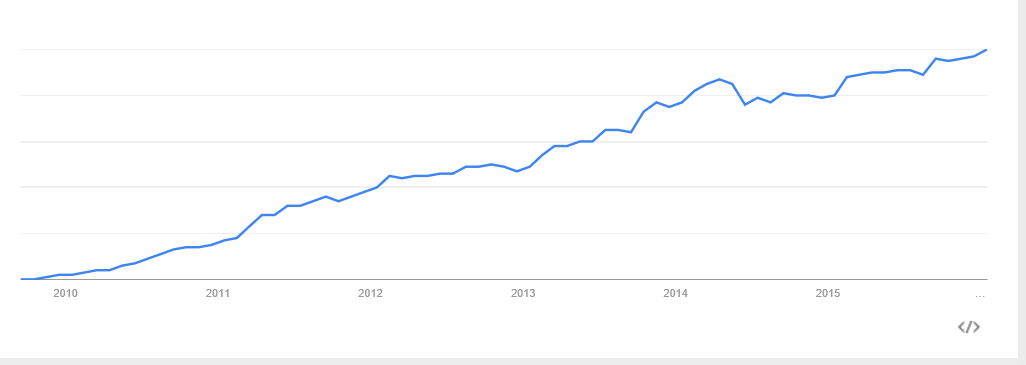
\includegraphics[width=0.7\linewidth]{figures/NodeJS.png}
	\caption{Steigerung der Suchanfragen für NodeJS. Datenquelle: Google Trends \cite{googleTrends:nodeJS}}
	\label{f:motivation:nodejs}
\end{figure}


Ein Großteil aller Webanwendungen ist in der Skriptsprache PHP geschrieben. 
So werden über 81\% aller Anwendungen damit geschrieben und ein demgegenüber verschwindend geringer Anteil von nur 0,1\% in JavaScript \cite{w3techs:serversidePLUsage}.
Dennoch stellt ein Grund sich näher mit dem MEAN Stack zu befassen die Tatsache dar, dass ein klarer Trend zu JavaScript erkennbar ist.
So ist das Interesse in den letzten Jahren enorm gestiegen wie auch in Abbildung \ref{f:motivation:nodejs} erkennbar ist.
Dort ist die Steigerung an Suchanfragen zu dem Thema NodeJS angegeben.
Google Trends liefert zwar keine absoluten Zahlen der Suchanfragen, jedoch lässt sich erkennen, dass die Anfragen sich in den letzten 5 Jahren linear steigern konnten. 
Auch ist der Bekanntheitsgrad von den anderen Komponenten wie MongoDB oder AngularJS stark gestiegen.
Selbst große Firmen wie RedBull oder Netflix setzen Teile davon ein.
Oftmals wird dies durch die verkürzte Entwicklungszeit zur Erstellung von Webanwendungen und durch die gesteigerte Performanz begründet.
Zudem hat es gewisse Vorteile für Unternehmen. So ist es beispielsweise leichter agile Methoden im Unternehmen einzuführen.
Meist werden Aufgaben in die Teile Frontend und Backend aufgeteilt und von unterschiedlichen Personen erarbeitet.
Frontendentwicklern, die sich mit den Technologien HTML, CSS und JavaScript auskennen und Backendentwicklern, die nur die serverseitigen Komponenten mit beispielsweise PHP und MySQL bearbeiten.
Da im MEAN Stack, NodeJS, Express und AngularJS auf JavaScript basieren und sogar MongoDB JavaScript ausführen kann, können nun die Aufgaben anderes aufgeteilt werden.
So ist es nicht mehr nötig nach Frondend und Backend zu trennen sondern die Aufgaben vertikal zu schneiden, wodurch jeder Entwickler alle Bereiche eines Features bearbeiten kann.
Vergleiche dazu das Elephant-Carpaccio von Alistair Cockburn \cite{cockburn:elephant}. 
Grund genug sich näher mit den einzelnen Komponenten zu beschäftigen.